%!TEX program = xelatex
% Note: this template must be compiled with XeLaTeX rather than PDFLaTeX
% due to the custom fonts used. The line above should ensure this happens
% automatically, but if it doesn't, your LaTeX editor should have a simple toggle
% to switch to using XeLaTeX.

\documentclass[
  aspectratio=169, % Uncomment to use an aspect ratio of 16:9 (160 mm by 90 mm)
  %aspectratio=43, % Uncomment to use an aspect ratio of 4:3 (128mm by 96mm)
  t, % Top align all slide content by default
  onlytextwidth, % Typeset content in columns at text width
  10pt, % Default font size, use 10pt for the 16:9 aspect ratio and 8pt for the 4:3 aspect ratio
]{beamer}

\usepackage{../ImperialTheme/beamerthemeImperial} % Use the Imperial theme

\def\imagefolder{../ImperialTheme/Images/}
\def\Rey{\text{Re}}
\title{Tries and errors} % Presentation title to appear on the title slide and left footers

\subtitle{} % Presentation subtitle to appear on the title slide

\author{Víctor Ballester} % Author name(s) to appear on the title slide

\date{\today} % Presentation date to appear on the title slide and right footers

\begin{document}

\begingroup
\setbeamercolor{background canvas}{bg=ICLBlue} % Slide background color
\setbeamercolor{title page title}{fg=white} % Title text color
\setbeamercolor{title page subtitle}{fg=white} % Subtitle text color
\setbeamercolor{author}{fg=white} % Author(s) text color
\setbeamercolor{date}{fg=white} % Date text color
\setbeamertemplate{title page}[logo]{\imagefolder/ICL_Logo_White.pdf} % Imperial logo color, use 'ICL_Logo_White.pdf' for white and 'ICL_Logo_Blue.pdf' for blue
\frame[plain, s]{\titlepage} % Output the title page with no footer ('plain') and vertically distributed text ('s')
\endgroup

\begin{frame}
	\frametitle{Stability plot with images}
	\centering
	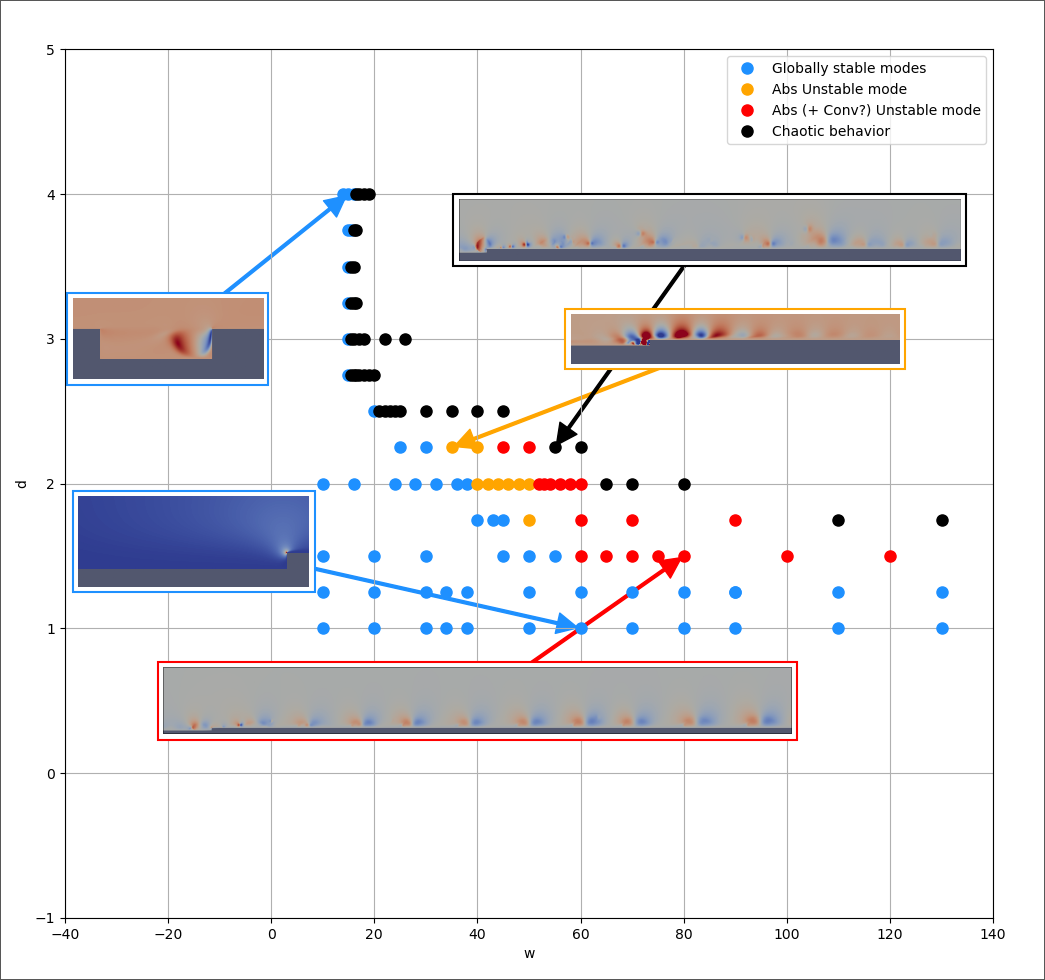
\includegraphics[width=0.5\linewidth]{Images/stabilitycurve.png}
\end{frame}
% At the end the parameters omega_r (= time frequency) and alpha_r (= wavelength) of the TS mode (from Orr-Sommerfeld eq) are correct and I am getting amplification in the amplitudes of the waves, as expected when blowing and suction. . I think last time I swapped them or anything even worse... Anyway the solver is correct. But in order to compute n(x) = max_omega m(x)

\begin{frame}
	\frametitle{Comments}
	\begin{itemize}
	  \item I realized I input the wrong frequency when blowing and suction, up to a factor of 1.72. Now I am redoing the computations. Could that explain that all the curves where clustered together?
	  \item I also try global stability analysis with the coupled approach, which worked (so far with low polynomial order), but it only does $kdim$ iterations and $kdim$ is bounded by 500 in the code. Why?
	\end{itemize}	
	\centering
	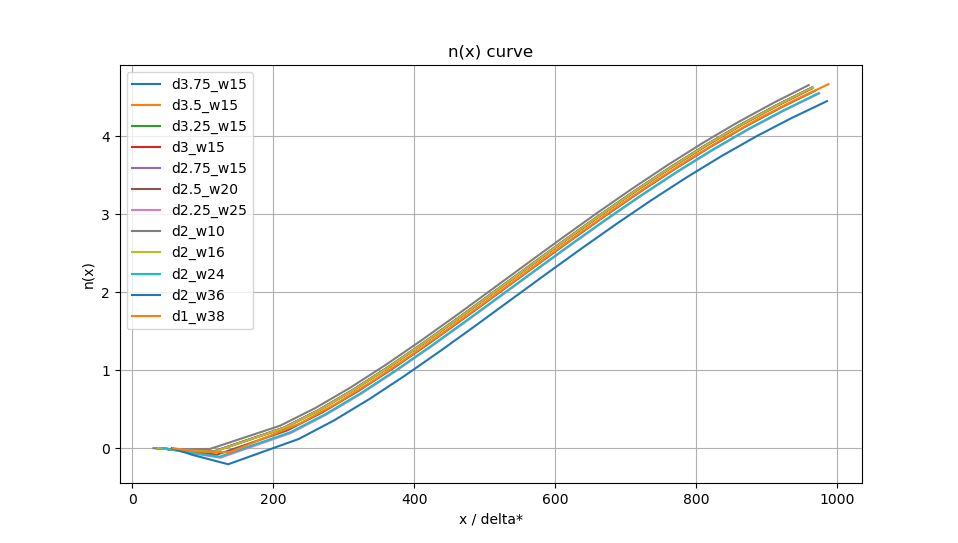
\includegraphics[width=0.5\linewidth]{Images/nfactorCurve.png}
\end{frame}
\end{document}
